\section{Convolutional Neural Networks}
\label{sec:intro}

CNNs are a strong architecture for computer vision tasks. We are going to explore its performance on image classification.

%-------------------------------------------------------------------------
\subsection{CNN architecture}
We desinged our CNN with
\begin{itemize}
	\item 4 convolutional layers with ReLU and Maxpooling
	\item 4 fully connected layers with drop-out and ReLU
	\item Residual connections to every one layers
	\item Use CrossEntropy as a loss function for optimization
	\item The size of convolutional filter size 3
\end{itemize}
In addition, the input of our CNN is resized to 128*128 as Caltech101 dataset has image sizes 100 to 300.
Also, the input image channel is 3(RGB) and it is amplified up to 256 through convolutional layers. For the output, it is reduced to 10 channels as we have 10 classed for the classification.
Above is our basic model. We tried to choose simplest yet high-performance model. Detailed reasons for our choice will be introduced below.

\subsection{Changing architecture}
First, the number of layers. We changed the number of layers from 3 to 5. As shown in \cref{fig:q4-2-layers}, the test accuracy of CNN is highest when the number of layers is 4. It may because, when CNN has 3 layers, it is not enough to capture features from images and when it has 5 layers, it may occur over-fitting due to many weights and gradient vanishing. Hence, we concluded that 4 layers are the best choice for the performance.

Next, we changed the size of kernel to 3, 5, and 7 to reveal its impact on CNN. As \cref{fig:q4-2-kernel} shows, the accuracy is highest when the kernel size is 3 and it decreases as the kernel size increases. It is because, when the kernel size is small, it is adequate to capture the details of images and when the size is big, it is good to perceive the global scene. However, as our image has 128*128 size, which is small, kernel size 3 is enough to extract useful feature of the image. other sizes are too big to recognize the features corresponding the image label.

Lastly, we conduct the experiments on connection between layers. There are three cases: no connection between layers, connect every 2 layers, connect every one layers. Since we have total 4 layers, the total number of connection is 0, 2, and 4. The test accuracy are shown in \cref{fig:q4-2-connection}. The accuracy is increases as the number of connection increases. It is because, the more connection CNN has, the more information it gets. By residual connection, CNN does not lose the information from initial layers thus it can learn more general information about images and its label.

\begin{figure}[htbp]
	\centering
	\begin{subfigure}[t]{0.3\linewidth}
		\centering
		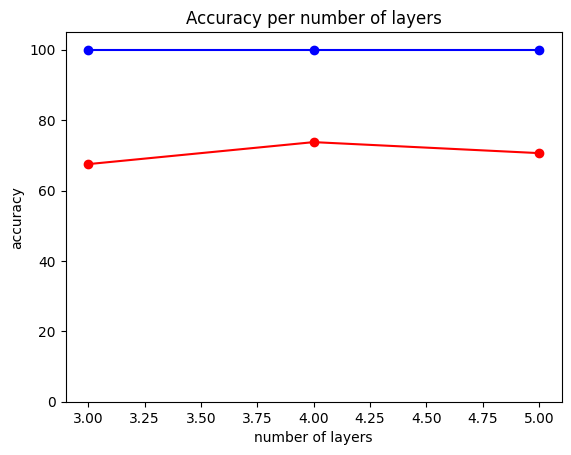
\includegraphics[width=\linewidth]{image/q4-2-layers.png}
		\caption{Accuracy according to layers}
		\label{fig:q4-2-layers}
	\end{subfigure}	
    \hfill
	\begin{subfigure}[t]{0.3\linewidth}
		\centering
		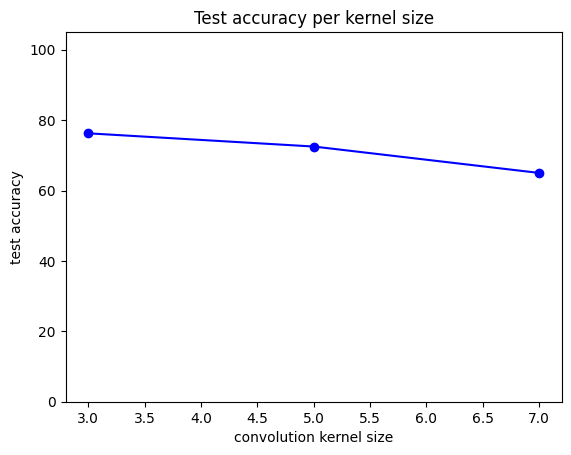
\includegraphics[width=\linewidth]{image/q4-2-kernel.png}
		\caption{Accuracy according to kernel size}
		\label{fig:q4-2-kernel}
	\end{subfigure}%
    \hfill
	\begin{subfigure}[t]{0.3\linewidth}
		\centering
		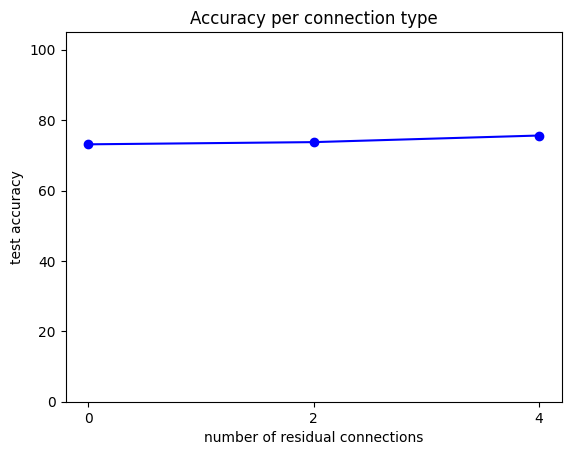
\includegraphics[width=\linewidth]{image/q4-2-connection.png}
		\caption{Accuracy according to connections}
		\label{fig:q4-2-connection}
	\end{subfigure}

	\caption{impact of changing architecture of CNNs}
	\label{fig:cnn_architecture}
\end{figure}

\subsection{Batch normalization}

\subsection{Generalization}
There are many method for Generalization of CNN. In this section, we are going to check the impact of drop-out and L2-regulization on weights(which is in Deep\_Learning\_intro Lecture Note pg.84) for the generalization.
We test our basic model which has drop-out, the basic model without drop-out, and the basic model with L2-regulization on weights.
Results are shown in \cref{table:generalization}. The model without drop-out has the lowest accuracy and the model with L2-regulization has the highest accuracy. 
This is because, drop-out randmly deactivate some neurons, so it helps model to avoid overfitting and be good at generalization. And L2-regulization helps model to avoid overfitting by regulize the size of weights.
Hence, it is natural result that the model with both drop-out and L2-regulization has the best performance.

\begin{table}[htbp]
	\centering
	\setlength{\tabcolsep}{10pt}
	\renewcommand{\arraystretch}{1.5}
	\begin{tabular}{|c||c|}
	\hline
	& accuracy  \\ \hline\hline
	original & 75.625  \\ \hline
	without dropout & 68.125  \\ \hline
	with L2-regularization term & 76.250  \\ \hline
	\end{tabular}
        \caption{Impact of generalization}
	\label{table:generalization}
\end{table}
	

\subsection{Loss function}
We use CrossEntropy, which is based on softmax function, as a loss function as usual. And compare it with SquaredHinge loss.

Using CrossEntropy for the loss function, we get 73.75\% accuracy. However, when we use SquaredHinge loss, we get 80.00\% accuracy. The accuracy with SquaredHinge loss is higher. This is because, as CrossEntropy is based on probability distribution and SquaredHinge loss is based on the margin between expected and real classes, SquaredHinge is better since our dataset is small. (which has only 10 classes) Because the dataset is small, it is hard to make an accurate probability distribution due to the law of large numbers. Hence, it is better to use direct borders and margins between classes.
Despite this reason, we adopted CrossEntropy as a basic loss function as it is widely used.

\subsection{Compressing CNN}
We conduct an experiment on compressing layers of CNN using truncated SVD. Since our model has 4 layers with rank 512, 128, 32, 10, we compress first two layers with 100(original), 75, 50, 25 percent each because last two layers are too small to compress, thus it might be cause the huge loss of data when they are compressed. The experiment result are shown in \cref{fig:cnn_svd}. Test accuracy and test time are both decreased as layers are more compressed. It is because, as weight matrix of layers become compressed, there remain less computation to get the result, so, the test time decreased. However, as the matrix is more compressed, it causes more data loss than the original weight matrix.

\begin{figure}[htbp]
	\centering
	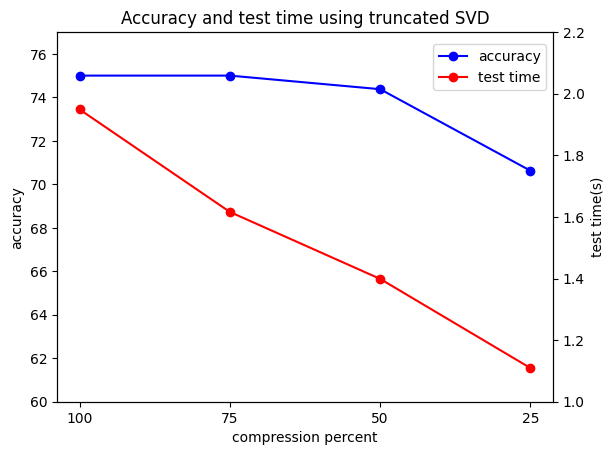
\includegraphics[width=0.5\linewidth]{image/q4-6-svd.png}
	\caption{Accuracy and test time using truncated SVD}
	\label{fig:cnn_svd}
\end{figure}

\subsection{Changing parameters}
We observe the influence of main hyper-parameters by experiments. We changed 3 parameters from base model: learning rate, batch size, and the number of epochs.

\cref{fig:q4-7-lr-train} and \cref{fig:q4-7-lr} indicates the result of varying learning rate. We changed learning rate to 0.00001, 0.0001, 0.0005, and 0.005. As shown in pictures, when the learning rate is 0.00001, the model doesn't converge sufficiently since it is too small, thus it can not reach the local minimum of loss during the given epochs. Conversely, when the learning rate is 0.0005 and 0.001, it vibrates too much until it reaches the convergence point. More specifically, amplitude of 0.001 is larger than 0.0005. This is because, the amount of moving is too big, so, the model oscillates near the local minimum largely. Therefore, we decided that learning rate = 0.0001 is the best for our model. Also, regarding the accuracy, the accuracy is higher when the learning rate is 0.0001 and less than this when the learning rate is smaller or bigger than 0.0001. It is because, if the learning rate is too small like 0.00001, it can not converge in the training time sufficiently. And if the learning rate is too big, it might pass through optimization point.

For the batch size, we trained our model with batch size from $2^1$ to $2^6$. Then we get highest accuracy when the batch size is 16 and the further away from 16, the lower the accuracy.(\cref{fig:q4-7-batch}) This is because, with small batch size, the model learn the feature distribution from small amount of data, the train result may be largely different from whole data distribution. On the other hand, if the batch size is too big, it is vulnerable for generalization and there exists a risk for over-fitting since the model learns statistics from a large amount of train data. Generally, batch size 32 is not big enough to cause the over-fitting, but, considering our whole train data is consist of 150 images, 32 is quite large number. Therefore, it is reasonable that batch size 16 is enough to get enough meaningful features while avoiding over-fitting.

Lastly, for the number of epochs, we use 75, 100, 125, 200 epochs and compared the result. Results are shown in \cref{fig:q4-7-epoch}. The accuracy was higher with 100 epochs. It is because, when the number of epoch is not enough, it can cause under-fitting while large amount of epochs can cause over-fitting during the training time.

\begin{figure}[htbp]
	\centering
	\begin{subfigure}{0.48\linewidth}
		\centering
		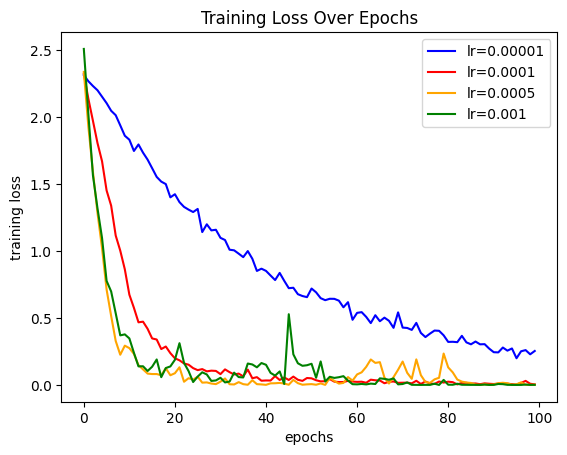
\includegraphics[width=\linewidth]{image/q4-7-lr-train.png}
		\caption{Train losses according to learning rates}
		\label{fig:q4-7-lr-train}
	\end{subfigure}%
	\hfill
	\begin{subfigure}{0.48\linewidth}
		\centering
		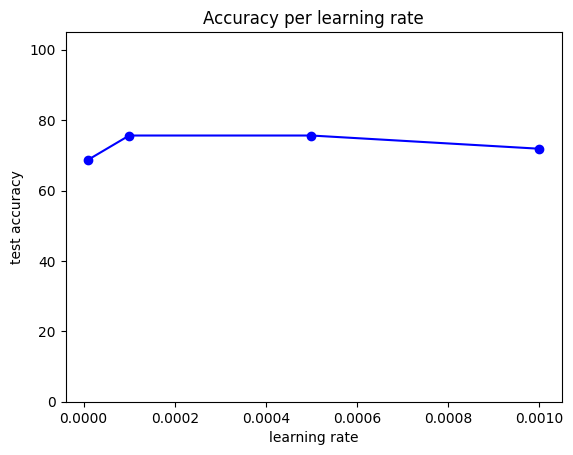
\includegraphics[width=\linewidth]{image/q4-7-lr.png}
		\caption{Accuracy according to learning rates}
		\label{fig:q4-7-lr}
	\end{subfigure}
	
	\begin{subfigure}{0.48\linewidth}
		\centering
		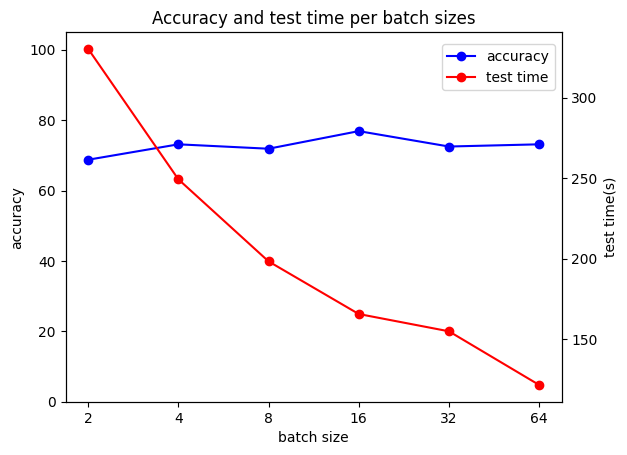
\includegraphics[width=\linewidth]{image/q4-7-batch.png}
		\caption{Accuracy according to batch sizes}
		\label{fig:q4-7-batch}
	\end{subfigure}
	\hfill
	\begin{subfigure}{0.48\linewidth}
		\centering
		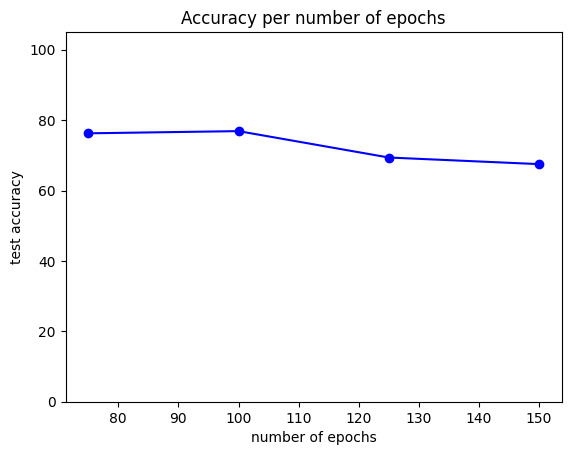
\includegraphics[width=\linewidth]{image/q4-7-epoch.png}
		\caption{Accuracy according to epochs}
		\label{fig:q4-7-epoch}
	\end{subfigure}
	\caption{Changing hyper-parameters of CNN}
	\label{fig:q2}
\end{figure}

\subsection{Pre-trained model}
In this section, we compare training methods: fine-tuning pre-trained model and training from scratch from random initialization. Since our CNN does not have pre-trained version because we have only one dataset for both training and test, we used pre-trained ResNet model(microsoft/resnet-50, trained with ImageNet) and custom it with our Caltech101 dataset. Due to the time limit, we only train it with 10 epochs. When we use pre-trained weights and fine-tuning them, we get 0.9933\% accuracy. And when we train the model from scratch, we get 0.2133\% accuracy which is lower than before. Based on this result, with the limited amount of time and resources, it is much better to use pre-trained model to get high performance. It may because, since we used pre-trained model with same task(image classification), trained weight is specialized for image classification even with different dataset. Therefore, fine-tuning using a custom dataset can achieve higher accuracy with fewer training epochs than train from scratch.

\subsection{Comparison with other methods}
Considering that our CNN have accuracy about 75\%, it is much better model than RF classifier and RF codebook on classifying Caltech101 dataset. (\cref{table:accuracy}) This may because, CNN can learn hierarchical features through layers, so, it can capture various characteristics of images. On the other hand, RF classifier and RF codebook use fixed method for extracting features from images, so they can only learn limited features.

\begin{table}[htbp]
	\centering
	\setlength{\tabcolsep}{6pt} % Adjust column spacing
	\renewcommand{\arraystretch}{1.5} % Adjust row height
	\resizebox{0.5\textwidth}{!}{ % Scale table to fit text width
		\begin{tabular}{|c||c|c|}
			\hline
			& Train Accuracy (\%) & Test Accuracy (\%) \\ \hline\hline
			K-means Codebook - RF Classifier & 99.50 & 68.5   \\ \hline
			RF Codebook - RF Classifier & 97.80 & 60.67  \\ \hline
			CNN & 100.00 & 75.625  \\ \hline
		\end{tabular}
	}
	\caption{Accuracy of Models}
	\label{table:accuracy}
\end{table}